\documentclass{beamer}[12pt]

\usepackage{setspace}
\usepackage[utf8]{inputenc}
\usepackage[T1]{fontenc}
\usepackage[english]{babel} %
\usepackage{csquotes}
%
\usepackage{graphicx}

%\usepackage{caption}
\usepackage[absolute,overlay]{textpos}
%\usepackage{subcaption}
\graphicspath{{/home/alain/Dropbox/Shared_TheseAlain/Figures/}}
%\graphicspath{{/home/alain.danet/Dropbox/Shared_TheseAlain/Figures/}}
\usepackage{tikz}
\usetikzlibrary{arrows,shapes,shapes.arrows}


\usetheme{Darmstadt}
%\usecolortheme[named=green]{structure}
\definecolor{vert}{rgb}{0,.5,0}
\usecolortheme[named=vert]{structure}
%\useoutertheme{sidebar}

\title{Plant-plant interactions: insights from an experimental and functional approach at the community level}
\author{Alain Danet}
\institute{Supervised by\\Susana Bautista \& Sonia Kefi}
\date{University of Montpellier\\ \today}

\begin{document}
   \tikzstyle{every picture}+=[remember picture]
   \everymath{\displaystyle}   
\begin{frame}
\titlepage
\end{frame}
\section{Introduction}
\subsection{Catastrophic shifts}


\begin{frame}\frametitle{Arid ecosystems}
\begin{columns}[t]

\begin{column}{0.5\textwidth}
\includegraphics[width=\textwidth]{high.jpg}
\end{column}

\begin{column}{0.5\textwidth}
\includegraphics[width=\textwidth]{low.jpg}
\end{column}
\end{columns}
\begin{center}
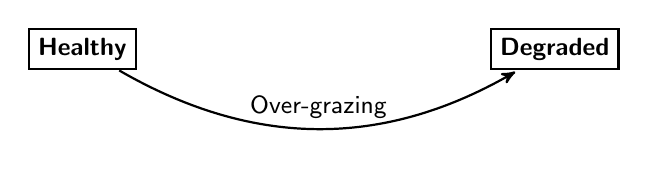
\begin{tikzpicture}[->,>=stealth',shorten >=1pt,auto,node distance=6cm,
                    thick,main node/.style={draw,font=\sffamily\small\bfseries}]

  \node[main node] (1) {Healthy};
  \node[main node] (2) [right of=1] {Degraded};

  \path[every node/.style={font=\sffamily\small}]
    (1) edge [bend right] node[above] {Over-grazing} (2);
 

\end{tikzpicture}
\end{center}
\end{frame}

\begin{frame}
\begin{figure}[!htb]
    \centering
    \begin{tikzpicture}
        \node[anchor=south west,inner sep=0] (image) at (0,0) {\includegraphics[scale=0.35]{Sole_fr.jpg}};
        \begin{scope}[x={(image.south east)},y={(image.north west)}]
            \node[anchor=south west,inner sep=0] (image) at (0.85,0.2) {\includegraphics[width=0.25\textwidth]{low.jpg}};
            \node[anchor=south west,inner sep=0] (image) at (0.19,0.75) {\includegraphics[width=0.25\textwidth]{high.jpg}};
        \end{scope}
    \end{tikzpicture}
\end{figure}

\end{frame}

\subsection{Facilitation}

\begin{frame}
\frametitle{Direct facilitation}

\begin{center}
Improving the local conditions
\vfill
\includegraphics[width=\textwidth]{goodpatch_badpatch.JPG}
\end{center}
\end{frame}

\begin{frame}
\frametitle{Indirect facilitation}

\begin{columns}
\begin{column}{0.5\textwidth}
\includegraphics[width=\textwidth]{quercus_buxus.pdf}\\
{\small \textit{Quercus pubescens \& Buxus sempervirens}}
\end{column}
\begin{column}{0.6\textwidth}
\begin{minipage}[t][0.3\textheight][t]{\textwidth}
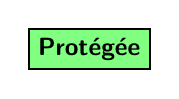
\begin{tikzpicture}[->,>=stealth',shorten >=1pt,auto,node distance=1cm,
                    thick,main node/.style={circle,draw,font=\sffamily\small\bfseries}]
  \node[main node, rectangle, fill=green!50] (nurse) {Protégée};
\end{tikzpicture}\\
Protection against herbivory
\end{minipage}
\begin{minipage}[b][0.3\textheight][b]{\textwidth}

\begin{tikzpicture}[->,>=stealth',shorten >=1pt,auto,node distance=1cm,
                    thick,main node/.style={circle,draw,font=\sffamily\small\bfseries}]

  \node[main node, fill=black, text=white, rectangle] (protege) {Protégée};
\end{tikzpicture}\\
No protection
\end{minipage}
\end{column}

\end{columns}

\end{frame}


\subsection{Stress Gradient Hypothesis}

\begin{frame}\frametitle{Concept}
\includegraphics[width=\textwidth]{SGH2.pdf} \\
\vfill
Shift in interaction importance along a stress gradient
\end{frame}

\begin{frame}\frametitle{How to measure it ?}
	\includegraphics[width=\textwidth]{Interaction_outcome.pdf}
\end{frame}

\subsection{Community level}
\begin{frame}\frametitle{Co-occurence observations}
	\includegraphics[width=\textwidth]{pairs_to_occurences.pdf}
\end{frame}
\begin{frame}\frametitle{We missed a step!}
	\begin{itemize}
		\item We infer the interaction strengths from co-occurence observations.
		\item Little is know about the effect of facilitation in the context of competition between saplings during etablishment.
		\item And obviously, different species answer differently to facilitation. 
	\end{itemize}
\end{frame}

\section{Research questions}
\begin{frame}\frametitle{Research questions}
	\begin{itemize}
		\item Can we predict the species responses to facilitation based on its functional group? 
		\item How do the species response to facilitation can be affected by the interspecific competition ?
		\item Can we infer the interaction strength from co-occurence observations ?
	\end{itemize}
\end{frame}

\subsection{Functional approach}
\begin{frame}\frametitle{Plant strategies}
	\includegraphics[width=\textwidth]{grime_englishv2.pdf}
\end{frame}
\begin{frame}\frametitle{Aim of the experiment}
	\includegraphics[width=\textwidth]{pairs_to_community.pdf}
	\vfill
	Build the bridge between the pair experiments and the co-occurence observations.
\end{frame}
\section{Methods}

\subsection{Experimental design}

\begin{frame}
	\includegraphics[width=\textwidth]{design_v2.pdf}
\end{frame}

\begin{frame}\frametitle{Complete design}
	\includegraphics[width=\textwidth]{design_number.pdf}
\end{frame}

\section{Predictions}

\begin{frame}
	\begin{center}
	\includegraphics[width=0.8\textwidth]{prediction.pdf}
	\end{center}
\end{frame}

\section{Merci!}
\begin{frame}
	\begin{center}
		Viva Santomera!
		\includegraphics[width=0.5\textwidth]{/home/alain/elise.jpg}

	\end{center}
\end{frame}
\end{document}
